\documentclass{standalone}

\usepackage{tikz}
\usetikzlibrary{angles,quotes}
\usepackage{amsmath,amssymb,amsfonts}

\usepackage{pgfplots}
\usepackage[makeroom]{cancel}
\usetikzlibrary{decorations.markings}
\definecolor{darkgreen}{rgb}{0.0, 0.42, 0.24}
\definecolor{amethyst}{rgb}{0.6, 0.4, 0.8}

\pgfplotsset{compat=newest}
\pgfplotsset{every axis/.append style={
                     tick label style={font=\footnotesize},
                 }}

\begin{document}
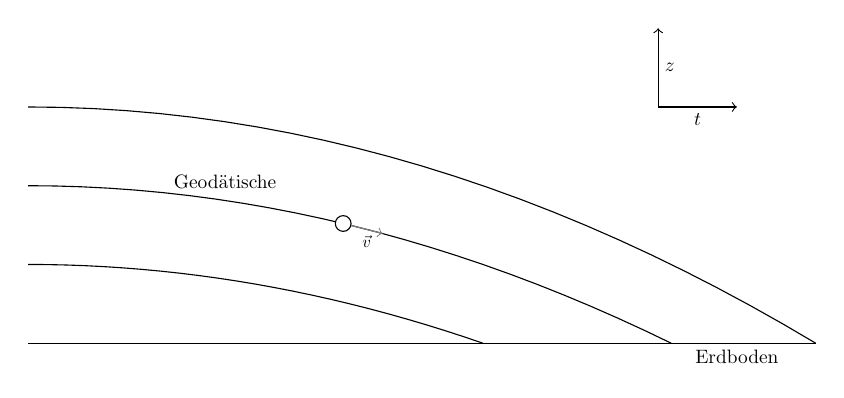
\begin{tikzpicture}
\draw[-](0,0)--(10,0) node[pos=0.9,below,scale=0.7]{Erdboden};
\draw[->](8,3)--(9,3) node[midway,below,scale=0.7]{$t$};
\draw[->](8,3)--(8,4) node[midway,right,scale=0.7]{$z$};

\draw[-,color=white](2,1.88)--(3,1.88)  node[midway,above,scale=0.7,color=black]{Geodätische};
\draw [domain=0:5.774] plot ({\x}, {-0.03*\x*\x+1});
\draw [domain=0:8.165] plot ({\x}, {-0.03*\x*\x+2});
\draw [domain=0:10] plot ({\x}, {-0.03*\x*\x+3});


\draw[fill=white] (4,1.52) circle[radius=0.1];
\draw[->,color=gray] (4.1,1.4957)--(4.5,1.3925) node[midway,below,scale=0.6,color=black]{$\vec{v}$};
\end{tikzpicture}
\end{document}